%% Figura 2 do exemplo do template — fluxograma do processo de controle.
%% Desenho de exemplo, para ser substituído pelo desenho do seu pedido.
%% Regenerar com:  pdflatex figura-2-fluxograma.tex
%% Art. 39, II — fluxogramas contêm descrições de atividades e/ou etapas.
\documentclass[border=6pt]{standalone}
\usepackage{tikz}
\usetikzlibrary{shapes.geometric, arrows.meta, positioning}
\begin{document}
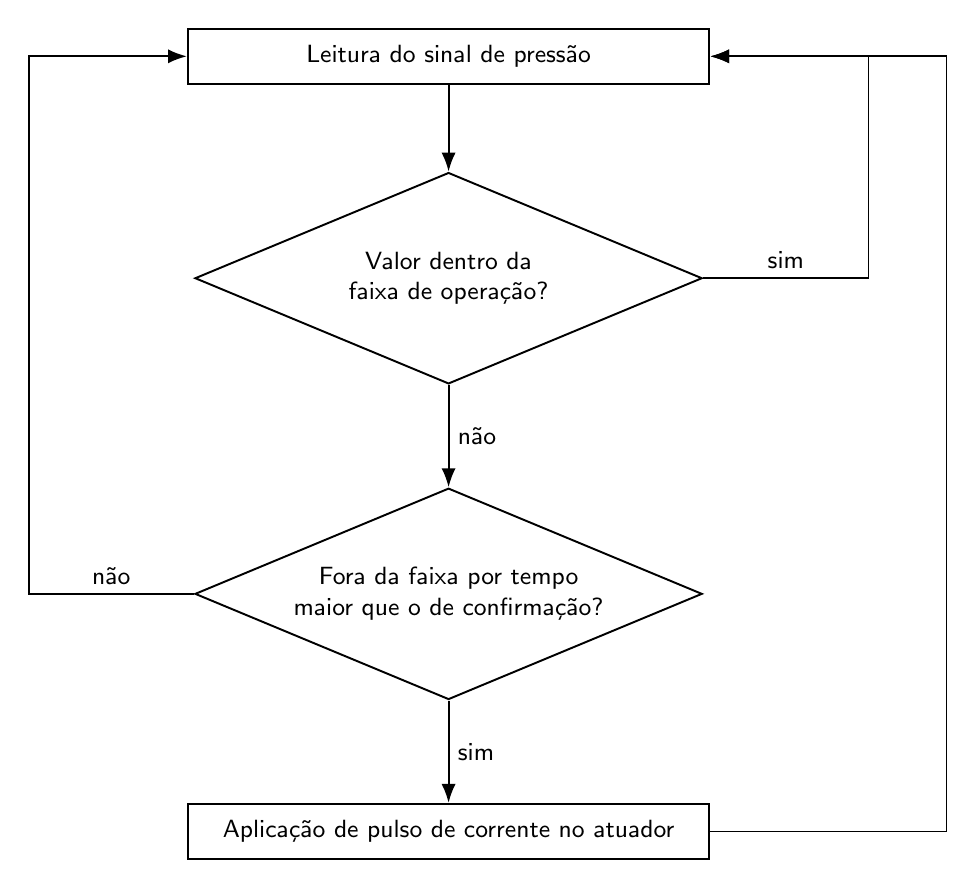
\begin{tikzpicture}[
    line width=0.7pt,
    font=\sffamily\small,
    node distance=1.1cm,
    caixa/.style={draw, rectangle, text width=6.2cm, align=center, inner sep=6pt},
    decisao/.style={draw, diamond, aspect=2.4, text width=4.6cm, align=center, inner sep=1pt},
    seta/.style={-{Latex[length=2.4mm]}}
]
    \node[caixa] (leitura) {Leitura do sinal de pressão};
    \node[decisao, below=of leitura] (faixa) {Valor dentro da faixa de operação?};
    \node[decisao, below=1.3cm of faixa] (tempo) {Fora da faixa por tempo maior que o de confirmação?};
    \node[caixa, below=1.3cm of tempo] (pulso) {Aplicação de pulso de corrente no atuador};

    \draw[seta] (leitura) -- (faixa);
    \draw[seta] (faixa) -- node[right, inner sep=3pt] {não} (tempo);
    \draw[seta] (tempo) -- node[right, inner sep=3pt] {sim} (pulso);

    \draw[seta] (faixa.east) -- node[above, inner sep=3pt] {sim} ++(2.1,0) |- (leitura.east);
    \draw[seta] (tempo.west) -- node[above, inner sep=3pt] {não} ++(-2.1,0) |- (leitura.west);
    \draw[seta] (pulso.east) -- ++(3.0,0) |- (leitura.east);
\end{tikzpicture}
\end{document}
